\section{Study of Trace Links}
\label{sec:approach}

\subsection{Impact of internal and external trace links}

	Creating trace links is expensive and error prone and in practice imperfect trace links are likely.
	Besides this, particularly design models such as UML models are often rather less used in practice\,\citep{Gorschek2014} and if present are probably not of the highest quality.
	Therefore, we are interested in how well TraceSEC performs in presence of imperfect trace links and planning artifacts (\ref{o4}).
	The overall question is whether lesser organized projects can still benefit from \appr{}.
	To understand the quality requirements on needed artifacts such as models and trace links, we are going to investigate how the accuracy of traceability links, i.e., connections within models and trace links between models and code, affect the importance rankings.

\subsubsection{Setup}
	To estimate the impact of imperfect traceability, we need to consider two types of trace links separately.
	First, internal links within artifacts (requirements \& design models), and second, external links between different artifacts (QM → requirements → design → code).
	The former indicates the quality of the artifacts produced, while the latter indicates how well trace links between different artifacts are created and maintained.
	Therefore, we considered these two types of trace links independently.



	To evaluate how robust TraceSEC is to imperfect trace links, we injected faults into the trace links by randomly deleting existing trace links or randomly creating additional trace links.
	Additions and deletions were performed independently, and we iteratively added and deleted between 0\% and 50\% of all trace links.
	After each change, we measured the quality of the prioritization in terms of correlation with the manual baseline.
	Since only detailed requirements and design models are available for iTrust, we performed this experiment only on this case study.



\subsubsection{Results}
%
	In  \autoref{tab:robustness} we show how much the correlation with the manual base line changed for the addition of false positives (fp) and deletions leading to false negatives (fn).
	When looking at the outcomes, missing external trace links severely impact the prioritization. However, false positives do not seem to be a  problem (it is often better to have a wrong trace link instead of no trace link).
	Therefore, external trace links must not be precise and internal trace links can make up for not accurate external trace links.
	On their own, internal trace links have only a low impact.
	Since the used models of iTrust were reverse engineered from the code and therefore only few information is added, this could be an explanation for this observed low impact but therefore high robustness.
	However, there is still a slight negative impact.

\begin{figure}

	\begin{subfigure}{\textwidth}
			\scriptsize
			\setlength{\tabcolsep}{1pt}
			\centering
			\begin{tabularx}{\textwidth}{>{\bfseries}r|XXXXXXXXXXXXXXXX}
					fp\textbackslash fn &	\textbf{0.0\%} &	\textbf{0.1\%} &	\textbf{0.2\%} &	\textbf{0.5\%} &	\textbf{1.0\%} &	\textbf{2.0\%} &	\textbf{5.0\%} &	\textbf{10.0\%} &	\textbf{15.0\%} &	\textbf{20.0\%} &	\textbf{25.0\%} &	\textbf{30.0\%} &	\textbf{35.0\%} &	\textbf{40.0\%} &	\textbf{45.0\%} &	\textbf{50.0\%} \\
					\hline
					0.0\%   &	0.00\% &	\rcolor{0.00} &	\rcolor{0.00} & \rcolor{0.00} & \rcolor{-0.35} &	\rcolor{-0.36} & \rcolor{-1.49} & \rcolor{-4.21} & \rcolor{-6.43} & \rcolor{-6.43} & \rcolor{-6.53} & \rcolor{-7.36} & \rcolor{-7.70} & \rcolor{-8.59} & \rcolor{-9.94} & \rcolor{-12.09} \\
					0.1\%   &	\rcolor{1.29} & \rcolor{1.23} & \rcolor{1.23} & \rcolor{0.99} & \rcolor{0.73} & \rcolor{0.41} & \rcolor{-0.72} & \rcolor{-2.02} & \rcolor{-2.28} & \rcolor{-2.48} & \rcolor{-3.65} & \rcolor{-2.81} & \rcolor{-4.21} & \rcolor{-3.32} & \rcolor{-3.09} & \rcolor{-5.35} \\
					0.2\%   &	\rcolor{2.06} & \rcolor{2.01} & \rcolor{2.04} & \rcolor{2.02} & \rcolor{2.01} & \rcolor{2.39} & \rcolor{0.28} & \rcolor{-1.55} & \rcolor{-1.84} & \rcolor{-1.71} & \rcolor{-2.01} & \rcolor{-1.65} & \rcolor{-3.01} & \rcolor{-2.84} & \rcolor{-3.22} & \rcolor{-2.76} \\
					0.5\%   &	\rcolor{2.25} & \rcolor{2.17} & \rcolor{2.17} & \rcolor{2.17} & \rcolor{2.17} & \rcolor{2.17} & \rcolor{1.73} & \rcolor{0.24} & \rcolor{-1.03} & \rcolor{-0.73} & \rcolor{-1.86} & \rcolor{-2.88} & \rcolor{-2.93} & \rcolor{-3.29} & \rcolor{-4.67} & \rcolor{-4.93} \\
					1.0\%   &	\rcolor{2.25} & \rcolor{2.17} & \rcolor{2.17} & \rcolor{2.17} & \rcolor{2.17} & \rcolor{2.25} & \rcolor{1.59} & \rcolor{0.92} & \rcolor{0.72} & \rcolor{0.22} & \rcolor{0.28} & \rcolor{0.08} & \rcolor{-1.36} & \rcolor{-1.45} & \rcolor{-1.56} & \rcolor{-1.17} \\
					2.0\%   &	\rcolor{2.25} & \rcolor{2.17} & \rcolor{2.16} & \rcolor{2.16} & \rcolor{2.16} & \rcolor{1.63} & \rcolor{1.58} & \rcolor{1.65} & \rcolor{0.60} & \rcolor{-1.61} & \rcolor{-1.59} & \rcolor{-0.88} & \rcolor{-0.77} & \rcolor{-0.91} & \rcolor{-0.81} & \rcolor{-0.80} \\
					5.0\%   &	\rcolor{2.43} & \rcolor{2.35} & \rcolor{2.35} & \rcolor{2.35} & \rcolor{2.35} & \rcolor{2.35} & \rcolor{2.25} & \rcolor{1.99} & \rcolor{0.50} & \rcolor{0.55} & \rcolor{0.18} & \rcolor{-0.37} & \rcolor{0.01} & \rcolor{-0.64} & \rcolor{-0.59} & \rcolor{-0.62} \\
					10.0\%  &	\rcolor{2.42} & \rcolor{2.33} & \rcolor{2.33} & \rcolor{2.33} & \rcolor{2.33} & \rcolor{2.18} & \rcolor{2.21} & \rcolor{2.60} & \rcolor{2.32} & \rcolor{2.01} & \rcolor{2.15} & \rcolor{1.57} & \rcolor{1.33} & \rcolor{1.17} & \rcolor{1.14} & \rcolor{1.13} \\
					15.0\%  &	\rcolor{2.42} & \rcolor{2.33} & \rcolor{2.33} & \rcolor{2.33} & \rcolor{2.33} & \rcolor{2.33} & \rcolor{2.33} & \rcolor{1.68} & \rcolor{1.24} & \rcolor{1.23} & \rcolor{1.10} & \rcolor{1.03} & \rcolor{1.03} & \rcolor{0.91} & \rcolor{0.91} & \rcolor{0.92} \\
					20.0\%  &	\rcolor{2.42} & \rcolor{2.33} & \rcolor{2.33} & \rcolor{2.33} & \rcolor{2.33} & \rcolor{2.33} & \rcolor{2.33} & \rcolor{1.97} & \rcolor{1.97} & \rcolor{1.97} & \rcolor{1.97} & \rcolor{2.11} & \rcolor{1.79} & \rcolor{1.54} & \rcolor{1.54} & \rcolor{1.54} \\
					25.0\%  &	\rcolor{2.42} & \rcolor{2.33} & \rcolor{2.33} & \rcolor{2.33} & \rcolor{2.33} & \rcolor{2.33} & \rcolor{2.17} & \rcolor{2.17} & \rcolor{2.42} & \rcolor{1.81} & \rcolor{1.81} & \rcolor{1.90} & \rcolor{1.90} & \rcolor{1.95} & \rcolor{1.95} & \rcolor{1.95} \\
					30.0\%  &	\rcolor{2.42} & \rcolor{2.33} & \rcolor{2.33} & \rcolor{2.33} & \rcolor{2.33} & \rcolor{2.33} & \rcolor{2.33} & \rcolor{2.30} & \rcolor{2.30} & \rcolor{2.18} & \rcolor{2.30} & \rcolor{2.44} & \rcolor{2.19} & \rcolor{2.17} & \rcolor{2.17} & \rcolor{2.17} \\
					35.0\%  &	\rcolor{2.42} & \rcolor{2.33} & \rcolor{2.33} & \rcolor{2.33} & \rcolor{2.33} & \rcolor{2.33} & \rcolor{2.33} & \rcolor{2.33} & \rcolor{2.07} & \rcolor{1.97} & \rcolor{1.97} & \rcolor{2.07} & \rcolor{2.07} & \rcolor{2.07} & \rcolor{2.07} & \rcolor{2.07} \\
					40.0\%  &	\rcolor{2.42} & \rcolor{2.33} & \rcolor{2.33} & \rcolor{2.33} & \rcolor{2.33} & \rcolor{2.33} & \rcolor{2.33} & \rcolor{2.30} & \rcolor{2.30} & \rcolor{2.18} & \rcolor{2.18} & \rcolor{2.42} & \rcolor{2.42} & \rcolor{2.41} & \rcolor{2.41} & \rcolor{2.41} \\
					45.0\%  &	\rcolor{2.42} & \rcolor{2.33} & \rcolor{2.33} & \rcolor{2.33} & \rcolor{2.33} & \rcolor{2.33} & \rcolor{2.33} & \rcolor{2.33} & \rcolor{2.33} & \rcolor{2.21} & \rcolor{2.21} & \rcolor{2.33} & \rcolor{2.33} & \rcolor{2.33} & \rcolor{2.33} & \rcolor{2.33} \\
					50.0\%  &	\rcolor{2.42} & \rcolor{2.33} & \rcolor{2.33} & \rcolor{2.33} & \rcolor{2.33} & \rcolor{2.33} & \rcolor{2.33} & \rcolor{2.33} & \rcolor{2.33} & \rcolor{2.21} & \rcolor{1.92} & \rcolor{1.92} & \rcolor{1.92} & \rcolor{1.73} & \rcolor{1.73} & \rcolor{1.73} \\
				\end{tabularx}

			\caption{Changes for external trace links between different artifacts.}
		\end{subfigure}

	\begin{subfigure}{\textwidth}
			\scriptsize
			\setlength{\tabcolsep}{1pt}
			\centering
			\begin{tabularx}{\textwidth}{>{\bfseries}r|XXXXXXXXXXXXXXXX}
					fp\textbackslash fn &	\textbf{0.0\%} &	\textbf{0.1\%} &	\textbf{0.2\%} &	\textbf{0.5\%} &	\textbf{1.0\%} &	\textbf{2.0\%} &	\textbf{5.0\%} &	\textbf{10.0\%} &	\textbf{15.0\%} &	\textbf{20.0\%} &	\textbf{25.0\%} &	\textbf{30.0\%} &	\textbf{35.0\%} &	\textbf{40.0\%} &	\textbf{45.0\%} &	\textbf{50.0\%} \\
					\hline
					0.0\% & 0.00\% & \rcolor{0.00} & \rcolor{0.00} & \rcolor{0.00} & \rcolor{0.00} & \rcolor{0.00} & \rcolor{0.02} & \rcolor{0.06} & \rcolor{0.06} & \rcolor{0.02} & \rcolor{0.03} & \rcolor{0.03} & \rcolor{0.00} & \rcolor{0.02} & \rcolor{0.07} & \rcolor{0.09} \\
					0.1\% & \rcolor{-0.01} & \rcolor{-0.01} & \rcolor{-0.01} & \rcolor{-0.01} & \rcolor{-0.01} & \rcolor{-0.01} & \rcolor{-0.01} & \rcolor{0.00} & \rcolor{-0.05} & \rcolor{-0.04} & \rcolor{-0.08} & \rcolor{-0.08} & \rcolor{-0.07} & \rcolor{-0.01} & \rcolor{0.04} & \rcolor{0.03} \\
					0.2\% & \rcolor{0.00} & \rcolor{0.00} & \rcolor{0.00} & \rcolor{0.02} & \rcolor{0.01} & \rcolor{0.01} & \rcolor{-0.03} & \rcolor{-0.04} & \rcolor{-0.02} & \rcolor{-0.03} & \rcolor{-0.03} & \rcolor{-0.03} & \rcolor{-0.03} & \rcolor{-0.06} & \rcolor{-0.06} & \rcolor{-0.06} \\
					0.5\% & \rcolor{0.00} & \rcolor{0.00} & \rcolor{-0.01} & \rcolor{-0.01} & \rcolor{-0.01} & \rcolor{-0.01} & \rcolor{-0.01} & \rcolor{0.00} & \rcolor{0.03} & \rcolor{0.05} & \rcolor{0.05} & \rcolor{0.05} & \rcolor{0.02} & \rcolor{-0.01} & \rcolor{-0.01} & \rcolor{-0.01} \\
					1.0\% & \rcolor{-0.01} & \rcolor{-0.01} & \rcolor{-0.01} & \rcolor{-0.01} & \rcolor{-0.01} & \rcolor{-0.01} & \rcolor{-0.01} & \rcolor{-0.02} & \rcolor{0.02} & \rcolor{0.02} & \rcolor{0.01} & \rcolor{0.01} & \rcolor{0.01} & \rcolor{0.01} & \rcolor{0.01} & \rcolor{0.01} \\
					2.0\% & \rcolor{-0.02} & \rcolor{-0.02} & \rcolor{-0.01} & \rcolor{-0.01} & \rcolor{-0.01} & \rcolor{-0.01} & \rcolor{-0.01} & \rcolor{-0.02} & \rcolor{-0.01} & \rcolor{-0.01} & \rcolor{0.03} & \rcolor{0.03} & \rcolor{0.03} & \rcolor{0.03} & \rcolor{0.03} & \rcolor{0.02} \\
					5.0\% & \rcolor{-0.02} & \rcolor{-0.02} & \rcolor{-0.02} & \rcolor{-0.02} & \rcolor{-0.02} & \rcolor{-0.01} & \rcolor{-0.01} & \rcolor{-0.02} & \rcolor{0.06} & \rcolor{0.06} & \rcolor{0.06} & \rcolor{0.06} & \rcolor{0.05} & \rcolor{0.05} & \rcolor{0.05} & \rcolor{0.05} \\
					10.0\% & \rcolor{-0.06} & \rcolor{-0.06} & \rcolor{-0.06} & \rcolor{-0.06} & \rcolor{-0.06} & \rcolor{-0.06} & \rcolor{-0.06} & \rcolor{-0.07} & \rcolor{-0.07} & \rcolor{-0.07} & \rcolor{-0.07} & \rcolor{-0.07} & \rcolor{-0.06} & \rcolor{-0.06} & \rcolor{-0.06} & \rcolor{-0.06} \\
					15.0\% & \rcolor{-0.06} & \rcolor{-0.06} & \rcolor{-0.06} & \rcolor{-0.06} & \rcolor{-0.06} & \rcolor{-0.06} & \rcolor{-0.06} & \rcolor{-0.06} & \rcolor{-0.07} & \rcolor{-0.07} & \rcolor{-0.06} & \rcolor{-0.03} & \rcolor{0.18} & \rcolor{0.18} & \rcolor{0.18} & \rcolor{0.18} \\
					20.0\% & \rcolor{-0.06} & \rcolor{-0.06} & \rcolor{-0.06} & \rcolor{-0.06} & \rcolor{-0.06} & \rcolor{-0.06} & \rcolor{-0.06} & \rcolor{-0.06} & \rcolor{-0.07} & \rcolor{-0.07} & \rcolor{-0.07} & \rcolor{-0.07} & \rcolor{-0.04} & \rcolor{-0.04} & \rcolor{-0.04} & \rcolor{-0.04} \\
					25.0\% & \rcolor{-0.06} & \rcolor{-0.06} & \rcolor{-0.06} & \rcolor{-0.06} & \rcolor{-0.06} & \rcolor{-0.06} & \rcolor{-0.06} & \rcolor{-0.10} & \rcolor{-0.10} & \rcolor{-0.10} & \rcolor{-0.11} & \rcolor{-0.11} & \rcolor{-0.14} & \rcolor{-0.14} & \rcolor{-0.09} & \rcolor{-0.09} \\
					30.0\% & \rcolor{-0.06} & \rcolor{-0.06} & \rcolor{-0.06} & \rcolor{-0.06} & \rcolor{-0.06} & \rcolor{-0.06} & \rcolor{-0.06} & \rcolor{-0.06} & \rcolor{-0.05} & \rcolor{-0.05} & \rcolor{-0.05} & \rcolor{-0.05} & \rcolor{-0.05} & \rcolor{-0.05} & \rcolor{-0.05} & \rcolor{-0.05} \\
					35.0\% & \rcolor{-0.06} & \rcolor{-0.06} & \rcolor{-0.06} & \rcolor{-0.06} & \rcolor{-0.06} & \rcolor{-0.06} & \rcolor{-0.06} & \rcolor{-0.06} & \rcolor{-0.06} & \rcolor{-0.06} & \rcolor{-0.06} & \rcolor{-0.06} & \rcolor{-0.06} & \rcolor{-0.06} & \rcolor{-0.06} & \rcolor{-0.06} \\
					40.0\% & \rcolor{-0.06} & \rcolor{-0.06} & \rcolor{-0.06} & \rcolor{-0.06} & \rcolor{-0.06} & \rcolor{-0.06} & \rcolor{-0.06} & \rcolor{-0.06} & \rcolor{-0.06} & \rcolor{-0.06} & \rcolor{-0.06} & \rcolor{-0.06} & \rcolor{-0.06} & \rcolor{-0.06} & \rcolor{-0.06} & \rcolor{-0.06} \\
					45.0\% & \rcolor{-0.06} & \rcolor{-0.06} & \rcolor{-0.06} & \rcolor{-0.06} & \rcolor{-0.06} & \rcolor{-0.06} & \rcolor{-0.06} & \rcolor{-0.06} & \rcolor{-0.06} & \rcolor{-0.06} & \rcolor{-0.06} & \rcolor{-0.06} & \rcolor{-0.06} & \rcolor{-0.06} & \rcolor{-0.06} & \rcolor{-0.06} \\
					50.0\% & \rcolor{-0.06} & \rcolor{-0.06} & \rcolor{-0.06} & \rcolor{-0.06} & \rcolor{-0.06} & \rcolor{-0.06} & \rcolor{-0.06} & \rcolor{-0.06} & \rcolor{-0.07} & \rcolor{-0.07} & \rcolor{-0.07} & \rcolor{-0.07} & \rcolor{-0.07} & \rcolor{-0.07} & \rcolor{-0.07} & \rcolor{-0.07} \\
				\end{tabularx}
			\caption{Changes for internal trace links within requirements and design models.}
		\end{subfigure}

	\small
	\setlength{\tabcolsep}{2pt}
	\scriptsize
	\begin{tabular}{|c|c|c|c|c|c|c|c|c|c|c|c|c|}
			\cellcolor{Red} < -10\% &
			\cellcolor{Red!75} < -8\% &
			\cellcolor{BurntOrange!75} < -6\% &
			\cellcolor{YellowOrange!75} < -4\% &
			\cellcolor{Goldenrod!85} < -2\% &
			\cellcolor{Yellow!85} < -1\% &
			\cellcolor{Yellow!40} -1\% < \& < 1\% &
			\cellcolor{ForestGreen!17} > 1\% &
			\cellcolor{ForestGreen!33} > 2\% &
			\cellcolor{ForestGreen!50} > 4\% &
			\cellcolor{ForestGreen!67} > 6\% &
			\cellcolor{OliveGreen!70} > 8\% &
			\cellcolor{OliveGreen!100} > 10\%\\
		\end{tabular}

	\caption{Average change in correlation with the manual baseline after adding (fp) or deleting (fn) trace links.}
	\label{tab:robustness}
\end{figure}

\begin{figure}
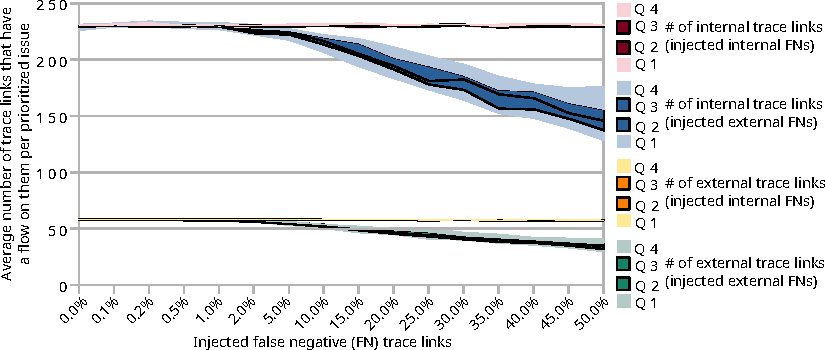
\includegraphics[width=.8\columnwidth]{figures/fns-edges.pdf}
\caption{Number of internal and external trace links used for prioritization dependent on the number of false negative trace links}
\label{fig:fnsEdges}
\end{figure}


	To better understand the results, we measured for the cases in which we only injected false negatives (FNs), i.e., deleting external or internal trace links how many of the edges in the flow network corresponding to them carry a flow when prioritizing an issue and how much flow this is per edge.
	As visible in \autoref{fig:fnsEdges}, the number of as well internal as external trace links that have a flow on them decreases with the number of deleted external trace links (FNs).
	Thereby, the number of internal trace links decreases stronger than the number of external trace links.
	If internal trace links are deleted, the numbers stay consistent.
	This fits to the results shown in \autoref{tab:robustness}, in which we also do not see a change for deleted internal trace links.
	Since as well the number of external trace links as internal trace links over which a flow is propagated decreases with increasing FNs, this implies that combinations of previously unused internal trace links cannot compensate missing external trace links to a notable extend.
	Instead, with deleted external trace links entire sub-graphs become uncreachable.
	When measuring the average flow across each trace link, we observed the same behavior as the number of trace links, implying also that the utilization of the used trace links, i.e., propagating additional flow over previously not saturated trace links, does not increase.


\begin{figure}
	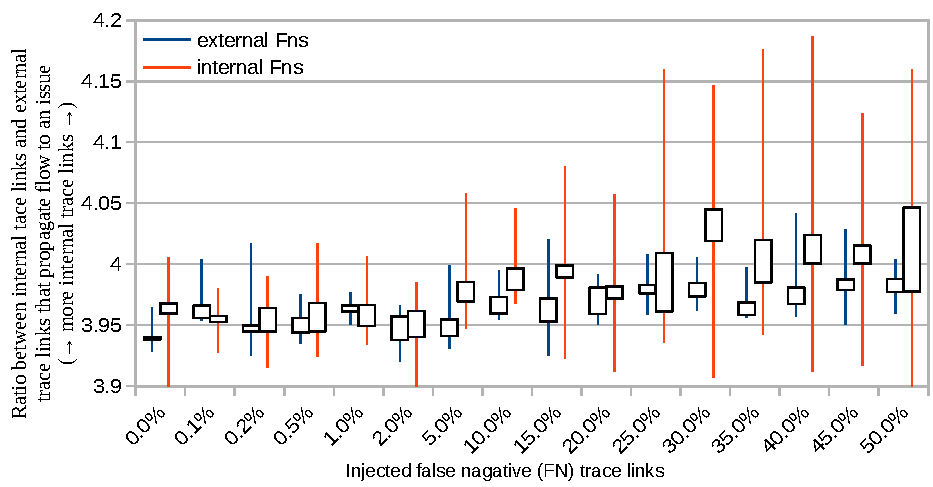
\includegraphics[width=.7\columnwidth]{figures/ratio-internal-to-external-tracelinks.pdf}
	\caption{Number of internal trace links to external trace links dependent on the number of false negative trace links}
	\label{fig:intVsExt}
\end{figure}

	When comparing the usage of external and internal trace links in the prioritization, meaning over which of them flow is propagated, we notice that the higher the number of false negative trace links gets, the more internal trace links are involved in the prioritization of an issue (see \autoref{fig:intVsExt}).
	While this trend can be observed to some extent for both, false negative internal trace links and external trace links, it is more pronounced for deleted external trace links.
	This indicates that internal trace links, e.g., design models or derived from code, play an essential role in distributing importance allowing for external trace links not immediately pointing to concrete issue locations, and allow the prioritization to also function to some extent for missing external trace links.


Overall, this experiment indicates that even low quality design models and imperfect trace links are sufficient for gaining benefit from TraceSEC.
Considering alternatives such as the SonarQube rule priorities for prioritizing issues, even in the worst case in which 50\% of all trace links have been deleted (a 12.09\% lower correlation coefficient), the prioritization of TraceSec still correlates stronger with the manual base line than the prioritization based on rule priorities (a correlation coefficient of .4041 for TraceSEC, while, according to \autoref{tab:correlations}, SonarQube rule priorities resulted only in .3023).
Therefore, we can conclude that it is likely that even lesser organized projects can benefit from TraceSEC.
Our deeper investigation of how internal and external trace links behave in this experiment suggests that it may be more beneficial to optimize external trace links than internal trace links.
However, since the two go hand in hand, artifacts containing internal trace links, such as requirements or design models, could be a means of optimizing external trace links between them.


\subsection{What are relevant trace links}

\begin{enumerate}
	\item Study which elements and types of trace links are on the flow edges with flow tokens.
	\item Randomly delete trace links and observe the deletion of which kind of trace links has huge impact.
\end{enumerate}
